%!TEX encoding = UTF-8 Unicode
%!TEX TS-program = pdflatex
% vim: spell spelllang=en_gb


%%%%%%%%%%%%%%%%%%%%%%%%%%%%%%%%%%%%%%%%%%%%%%%%%%%%%%%%%%%%%%%%%%%%%%%%%%%%%%%%%%%%%%%%%%%%%%
%
% This extended-abstract version of this paper was submitted, accepted and presented to/at the CLARIN conference 2024. 
% The post-proceedings paper is a work in progress and still pending submission and further peer review.
%
%%%%%%%%%%%%%%%%%%%%%%%%%%%%%%%%%%%%%%%%%%%%%%%%%%%%%%%%%%%%%%%%%%%%%%%%%%%%%%%%%%%%%%%%%%%%%%%%5

\documentclass[a4paper,11pt]{article}
\usepackage{CLARIN2024}
% - - - - - - - IMPORTANT - - - - - - - -
% The next three lines allow XeLaTeX, graphics import and hyperlinks, set font and language
%\usepackage{xltxtra,polyglossia,graphicx,hyperref}
%\setmainfont[Mapping=tex-text]{Times}
%\setdefaultlanguage{english}
% If for some reason the above three lines are not compatible with your LaTeX installation,
% comment out the above three instructions and uncomment the following four instead:
\usepackage{times}
\usepackage{url}
\usepackage{latexsym}
\usepackage{hyperref}
\usepackage{graphicx}
\usepackage{placeins}
\usepackage[english]{babel}
\usepackage{csquotes}
\usepackage{listings}
\usepackage{xcolor}
\usepackage[
    backend=biber,
    style=apa,
    natbib=true,
    ]{biblatex}
\addbibresource{tooldiscovery.bib} % add your own bibliography into the format provided in this file


% JSON highlighting, copied from https://tex.stackexchange.com/questions/83085/how-to-improve-listings-display-of-json-files
\definecolor{eclipseStrings}{RGB}{42,0.0,255}
\definecolor{eclipseKeywords}{RGB}{127,0,85}
\colorlet{numb}{magenta!60!black}
\lstdefinelanguage{json}{
    basicstyle=\normalfont\ttfamily\footnotesize,
    commentstyle=\color{eclipseStrings}, % style of comment
    stringstyle=\color{eclipseKeywords}, % style of strings
    numbers=left,
    numberstyle=\scriptsize,
    stepnumber=1,
    numbersep=8pt,
    showstringspaces=false,
    breaklines=true,
    frame=lines,
    string=[s]{"}{"},
    comment=[l]{:\ "},
    morecomment=[l]{:"},
    literate=
        *{0}{{{\color{numb}0}}}{1}
         {1}{{{\color{numb}1}}}{1}
         {2}{{{\color{numb}2}}}{1}
         {3}{{{\color{numb}3}}}{1}
         {4}{{{\color{numb}4}}}{1}
         {5}{{{\color{numb}5}}}{1}
         {6}{{{\color{numb}6}}}{1}
         {7}{{{\color{numb}7}}}{1}
         {8}{{{\color{numb}8}}}{1}
         {9}{{{\color{numb}9}}}{1}
}


%\setlength\titlebox{5cm}

% You can expand the titlebox if you need extra space
% to show all the authors. Please do not make the titlebox
% smaller than 5cm (the original size); we will check this
% in the camera-ready version and ask you to change it back.

%\usepackage{covington} % if needed, for linguistic examples

\title{FAIR Tool Discovery: an automated software metadata harvesting pipeline for CLARIAH}

% - - - - - - - IMPORTANT - - - - - - -
% Leave the author information empty until your paper has been accepted 

% Uncomment the following line ONLY if you need two author rows
%\setlength\titlebox{80mm} 

\author{Maarten van Gompel \\
  KNAW Humanities Cluster \\
  Amsterdam, the Netherlands \\
  {\tt proycon@anaproy.nl} \And % if needed: this makes a second column
  Menzo Windhouwer \\
  KNAW Humanities Cluster \\
  Amsterdam, the Netherlands \\
  {\tt menzo.windhouwer@di.huc.knaw.nl}
%  Department (optional)\\
%  University Name without city \\
%  City, Country \\
% {\tt email@domain} \\
% \AND % if needed: this makes a second row
%  Third Author \\
%  Department (optional)\\
%  University of City, Country \\
%  {\tt email@domain} \\\And
%  Fourth Author \\
%  Department (optional)\\
%  University Name without city \\
%  City, Country \\
%  {\tt email@domain} \\
} 

\date{}

\begin{document}
\maketitle
\begin{abstract}
  We present the Tool Discovery pipeline, a core component of the CLARIAH
    infrastructure in the Netherlands. This pipeline harvests software metadata
    from the source, detects existing heterogeneous metadata formats already in
    use by software developers, and converts them to a single uniform representation
    based on schema.org and codemeta. The resulting data is then made available
    for further ingestion into other user-facing catalogue/portal systems. 
\end{abstract}

\section{Introduction} \label{intro}

% - - - - - - - IMPORTANT - - - - - - -
% The following footnote without marker is needed for the camera-ready
% version of the paper.
% Comment out the instructions (first text) and uncomment the 8 lines
% under "final paper" for your variant of English.
%
\blfootnote{
    %
    % for review submission
    %
    %\hspace{-0.65cm}  % space normally used by the marker
This work is licenced under a Creative Commons Attribution 4.0 International Licence. Licence details: {http://creativecommons.org/licenses/by/4.0/}
    % % final paper: en-uk version (to license, a licence)
    %
    % \hspace{-0.65cm}  % space normally used by the marker
    % This work is licensed under a Creative Commons
    % Attribution 4.0 International Licence.
    % Licence details:
    % {http://creativecommons.org/licenses/by/4.0/}
    %
    % % final paper: en-us version (to licence, a license)
    %
    % \hspace{-0.65cm}  % space normally used by the marker
    % This work is licenced under a Creative Commons
    % Attribution 4.0 International License.
    % License details:
    % {http://creativecommons.org/licenses/by/4.0/}
}

Software is indispensable in a lot of modern-day research, including in sectors
such as the Humanities and Social Sciences that may have traditionally been
less focused on information technology. It is also appreciated more and more as
valid research output, alongside more conventional output such as academic
publications, presentations, and datasets. Scholars often have a need for
research software to do their research efficiently.

For scholars it is therefore important to be able to find and identify tools suitable for
their research, we call this process \emph{tool discovery}. We define
\emph{tool} here and throughout this paper to broadly refer to any kind of
software, regardless of the interface it offers and the audience it targets.
The scholar's requirement to find tools is reflected in the letter \textsc{F}
for \emph{Findable} in the ubiquitous acronym \textsc{FAIR} \footnote{Findable,
Accessible, Interoperable and Reusable} that has received a lot of attention in
recent years in academic circles. The term is often adopted to promote quality and
sustainability in research software \citep{FAIR}. In order to find tools,
researchers must have access to catalogues that relay \emph{accurate} software
metadata.

There is no shortage in existing initiatives in building such catalogues; many
research groups, projects or institutes have some kind of website featuring
their tools. Aggregation of software metadata from multiple sources is also not
new. CLARIN itself already does this in the CLARIN Virtual Language
Observatory\footnote{\url{https://vlo.clarin.eu}} \citep{VLO}, and DARIAH in
the SSHOC Open Marketplace\footnote{\url{https://marketplace.sshopencloud.eu/}}
. However, the system we describe in this paper is not an attempt to build
another catalogue. We developed a generic pipeline that harvests software
metadata from the software's source, leveraging various existing metadata
formats, and converting those to a uniform linked open data representation.
This data can then be used to feed catalogues.

\section{The need for high-quality metadata}
\label{sec:need}

Unlike most digital data, software is uniquely characterised as a constantly
moving target rather than a static deliverable entity. Releases at different
points in time address bugs, security vulnerabilities, or add new features.
Moreover, software lives not in isolation, but in connection to other software;
its dependencies. Updates are needed to adapt to changes in its runtime
environment.

For software metadata to be informative in this dynamic setting, it needs to
reflect this moving target and explicitly link to a particular version of the
software. This also facilitates provenance keeping and scientific
reproducibility. Furthermore, metadata should convey information about the stage of
development the software is in and the level of support an end-user may expect.
The user would be wise to exercise caution in adopting software that is
unmaintained and unsupported. In practice we often find this information
lacking and come across catalogues that were manually compiled once but rarely
updated since.

The need for accurate up-to-date metadata goes hand-in-hand with the need for
\emph{complete} metadata. If vital details are missing, the
end-user may not be able to make an informed judgment.

A common pitfall we have observed in practice is that metadata is often
manually collected at some stage and published in a catalogue, but never or
rarely updated or revised. In best case, the software has moved on and the
metadata covers a mere subset, in worst case, the software or the entire
catalogue is unmaintained and out of date.

\section{Bottom-up harvesting from the source}

What we propose is a \emph{fully automated} pipeline where software metadata is
kept at the source, i.e. alongside the software source code, and
\emph{periodically} harvested from there. This is in contrast to approaches
where metadata primarily resides in an intermediate system that is manually
constructed or curated, which is a common approach for many
software catalogues\footnote{for example, \url{https://research-software-directory.org/}
offers such a platform. Metadata can often be exported via OAI-PMH.}. Our approach has a number of important advantages:

\begin{enumerate}

\item
Source code is often already accompanied by software metadata in existing
schemas because many programming language ecosystems already either require or
recommend this. Our aim is to avoid any duplication of metadata and
\emph{reuse} these existing sources to the maximum extent possible.

Consider
for example \texttt{pyproject.toml} or \texttt{setup.py} for Python projects,
\texttt{package.json} for javascript/npm/nodejs projects, \texttt{pom.xml} for
Java/Maven and \texttt{Cargo.toml} for Rust. Aside from these, valuable machine
parsable metadata may be extracted from other conventional files such as a \texttt{LICENSE}
file or a \texttt{README.md} file. The latter often contains machine-interpretable
badges. Badges are small images often included on top of the README to express certain properties of the software, such as links to
documentation, continuous integration services, development status, packaging
status. Research software developers also often include a \texttt{CITATION.cff}\footnote{\url{https://citation-file-format.github.io/}} file which we can automatically parse for metadata. All these different
sources may be present and can be recombined in our harvesting process.

\item 
  Source code 
  is typically held in a version control system (usually git) and published in 
  forges such as Github, Gitlab, Bitbucket, Codeberg or Sourcehut.
  This solves versioning issues and ensures metadata can exactly describe the version alongside which it is stored. It also enables the 
  harvester to properly identify the latest stable release, provided some kind of industry-standard versioning system like semantic versioning is adhered to.
  Software forges themselves may also provide an Application Programming Interface (API) that may serve as an extra source to find software metadata (e.g. descriptions, keywords, links to issue trackers and/or continuous integration services).
\item 
  The developers of the tool have full control and authorship over their metadata. There are no middlemen.
\item 
  Software forges were designed precisely for collaboration on open source software development, so mechanisms for any
  third party to amend or correct the metadata are already in place (e.g. via a pull/merge request or patch via e-mail).
  So while developers retain full authorship, this does not mean outside contribution and curation is not possible.
\end{enumerate}

We do not harvest any metadata from intermediaries. By that we mean that we do
not use other catalogues as sources (e.g. via the aforementioned OAI-PMH
endpoints), only the software source itself. Using intermediaries would defeat
our philosophy. We do have one extra input source for harvesting: In case the
tool in question is Software as a Service (SaaS), i.e. a web-application,
web-service, or website, we harvest not only its software source code, but also
its web endpoint and attempt to automatically extract metadata from there. We
make a clear distinction between the software source code, software instances
(executables) you can run locally, and software instances offered as a service
via the web. Formally, the software source code has no knowledge when, where,
and by whom it may be deployed, neither locally on some user's computer nor as
a service on some server. This link is therefore established at an independent
and higher level. In the resulting metadata, there will be an explicit link
between the source code and \emph{applications} of that source
code\footnote{Applications are instances of the source-code in executable form
after build and deployment and may also refer to availability as a service over
a network}. The sources for harvesting source repositories and web endpoints
(both effectively just URLs) are the only input that needs to be manually
provided to our harvesting system, we call this the \emph{source registry}.
This is the higher level we referred to earlier. We keep the source registry in
a simple git repository containing very minimalistic configuration files (one
yaml file per tool). This is also the only point in our pipeline where there is
the possibility for a human curator to decide whether or not to include a tool.

Usage of such a manually curated source registry means that, for this project,
automatic discovery of tools is not in scope. That is, we do not actively crawl
the web in search for tools that might or might not fit a certain domain. Some
interpret the term `tool discovery' to also include such functionality, but we
do not. Such a step, however, can be envisioned as a separate step prior to
execution of our pipeline.

\section{A unified vocabulary for software metadata}

The challenge we are facing is primarily one of mapping multiple heterogeneous
sources of software metadata to a unified vocabulary. Fortunately, this is an
area that has been explored previously in the CodeMeta
project\footnote{\url{https://codemeta.github.io}}. They developed a generic
vocabulary for describing software source code, extending schema.org vocabulary
and contributing their efforts back to them. Moreover, the CodeMeta project
defines mappings, which they call \emph{crosswalks}, between their vocabulary and many existing
metadata schemes, such as those used in particular programming languages
ecosystems or by particular package managers.

Schema.org and CodeMeta are both linked open data (LOD)
vocabularies\footnote{i.e. building upon RDF and being retrievable over HTTP},
and codemeta is canonically serialised to a
JSON-LD\footnote{\url{https://www.w3.org/TR/json-ld/}} file which makes it
easily parsable for both machine and human alike. This \texttt{codemeta.json}
file can be kept under version control alongside a tool's source code. A 
rather minimal example of a such a file is shown below:

\begin{lstlisting}[language=json] 
{
    "@context": [
        "https://w3id.org/codemeta/3.0",
        "http://schema.org",
    ],
    "@id": "https://example.org/mysoftware",
    "@type": "SoftwareSourceCode",
    "identifier": "mysoftware",
    "name": "My Software",
    "author": {
        "@type": "Person", 
        "givenName": "John",
        "familyName": "Doe"
    },
    "description": "My software does nice stuff",
    "codeRepository": "https://github.com/someuser/mysoftware",
    "license": "https://spdx.org/licenses/GPL-3.0-only",
    "developmentStatus": "https://www.repostatus.org/#active",
    "thumbnailUrl": "https://example.org/thumbnail.jpg"
}
\end{lstlisting}

The developer has a choice to either run our harvester and converter themselves and
commit the resulting codemeta file, or to not add anything and let the harvester
dynamically reconstruct the metadata every harvest cycle.

The convention to add a \texttt{codemeta.json} file alongside the source code
was established by the CodeMeta project. In addition to this, we define another
method that is specific for our metadata harvester: Developers can add a
\texttt{codemeta-harvest.json} file instead of \texttt{codemeta.json}. Whereas
\texttt{codemeta.json} by definition contains the complete metadata, the
\texttt{codemeta-harvest.json} file contains an arbitrary subset and is used to
supplement any automatically harvested metadata. This allows developers to rely
on the harvester for most fields, without having to run it themselves, but
still allows them to provide additional manual metadata. All these different
options ensure that developers themselves can choose precisely how much control
to exert over the metadata and harvester. It allows us to accommodate both
projects that aren't even aware they're being harvested, as well as projects
that want to fine-tune every metadata field to their liking, effectively
rendering most of our periodic harvester out of work at run-time.

\subsection{Additional Vocabularies}

We link to various other linked open data vocabularies, listed below. Most of these are
formulated as SKOS\footnote{\url{https://www.w3.org/TR/skos-reference/}}
vocabularies.

\begin{itemize}
\item \textbf{repostatus.org}\footnote{\url{https://repostatus.org}} -- \emph{Development Status} -- The repostatus.org project allows developers to express usability and development/support status of a project.
A LOD (SKOS) version of this vocabulary was developed in the scope of this project and contributed back to the repostatus project.
\item \textbf{SPDX}\footnote{\url{https://spdx.dev}} -- \emph{Open-source software licenses} -- The Software Package Data Exchange project is a Linux Foundation project that defines, amongst other things, open source software licenses. It is widely used, e.g. by package managers. 
\item \textbf{TaDiRaH}\footnote{\url{https://vocabs.dariah.eu/tadirah/}} -- \emph{Research activities} -- The TaDiRAH vocabulary ``classifies and categorizes the activities that comprise digital humanities'' \citep{TADIRAH} with the aim to help scholars group and identify projects that share certain commonalities.
We adopt this vocabulary to describe the research activities a software tool can be used for. Example of some top-level categories in this vocabulary are `Analyzing', `Capturing', `Creating`, `Enriching'. An example of a deeper-level category that is particularly common in language resources such as those 
seen in CLARIN is for example `Enriching $\rightarrow$ Annotating $\rightarrow$ Named Entity Recognition'.
\item \textbf{NWO Research Domains}\footnote{\url{https://www.nwo.nl/en/nwo-research-fields}} -- NWO is the Dutch Research Council. They define several research fields that are used for official grant applications. As CLARIAH is a Dutch project, we use this vocabulary to express the research domain a tool is used for. A LOD (SKOS) version of this vocabulary was developed in the scope of this project.
\end{itemize}

The first two vocabularies are generic enough to be applicable to almost all
software projects, we strongly recommend their usage. The latter two may be
more constrained to research software as developed in CLARIAH and CLARIN. In
your projects, you can adopt whatever you find suits your needs best, the power to mix and
match is at the heart of linked open data after all.

Moreover, we formulated some of our own extensions on top of codemeta and
schema.org:

\begin{itemize}
\item \textbf{Software Types}\footnote{\url{https://github.com/SoftwareUnderstanding/software_types}}
-- Software comes in many shapes and forms, targeting a variety of
audiences with different skills and needs. We want
software metadata to be able to accurately express what type(s) of
interface their software provides. The schema.org vocabulary
distinguishes \texttt{softwareApplication}, \texttt{WebApplication},
\texttt{MobileApplication} and even \texttt{VideoGame}. This covers
some interfaces from a user-perspective, but is not as extensive nor as
fine-grained as we would like yet. Interface types from a more
developer-oriented perspective are not formulated. We therefore define
additional classes such as \texttt{DesktopApplication} (software
offering a desktop GUI), \texttt{CommandLineApplication},
\texttt{SoftwareLibrary} and others in this add-on vocabulary.
\item \textbf{Software Input/Output Data}\footnote{\url{https://github.com/SoftwareUnderstanding/software-iodata}}
-- This minimal vocabulary defines just two new properties that allows for software metadata to
express what kind of data it consumes (e.g. takes as input) and what
kind of data it produces (e.g. output). It does not define actual data types because schema.org already has 
classes covering most common data types (e.g. \texttt{AudioObject}, \texttt{ImageObject}, \texttt{VideoObject}, \texttt{TextDigitalDocument}, etc...) and properties
like \texttt{encodingFormat} to tie these to MIME-types or \texttt{inLanguage} to tie it to natural languages.

Do note that describing a full API is explicitly out of scope for our project.
A full API description would describe exactly which function or
web-endpoints take and return what data. Although this too can be
considered a type of metadata, such functionality goes beyond what we consider
the primary software metadata which end-users need to make a informed
decision regarding the suitability of a tool for their ends. Other
existing projects such as the OpenAPI
Initiative\footnote{\url{https://www.openapis.org}} delve into this realm 
for Web APIs. For software libraries there are 
various existing API documentation generators\footnote{e.g. doxygen, sphinx,
rustdoc, etc...} that derive documentation directly from the source
code in a formalised way. We do not intend to duplicate those efforts.
\end{itemize}

\section{Architecture}

The full architecture of our pipeline is illustrated schematically in
Figure~\ref{fig:architecture}. Although we demonstrate this in the context of the
CLARIAH project, the underlying technology is generic and can also be used for
other projects.

\begin{figure}[h]
\begin{center}
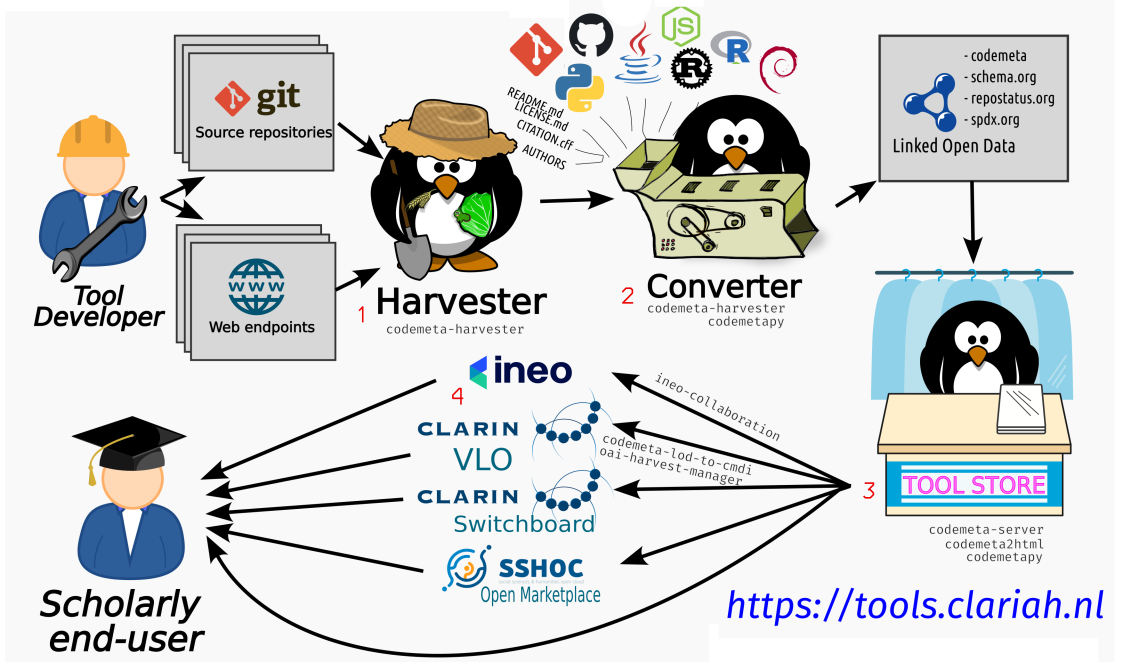
\includegraphics[width=14.0cm]{architecture.png}
\caption{The architecture of the CLARIAH Tool Discovery pipeline. Key steps are numbered in red and referenced in the text.}
\label{fig:architecture}
\end{center}
\end{figure}

Using the input from the source registry, our
\emph{harvester}\footnote{\url{https://github.com/proycon/codemeta-harvester}, marked with a red 1 in Figure~\ref{fig:architecture}} (1) \citep{CODEMETAHARVESTER} fetches all the git
repositories and queries any service endpoints. It does so at regular intervals
(e.g. once a day). This ensures the metadata is always up to date. When the
sources are retrieved, it looks for different kinds of metadata it can identify
there and calls the converter (2) powered by codemetapy\footnote{\url{https://github.com/proycon/codemetapy}} \citep{CODEMETAPY}
to turn and combine these into a single codemeta representation. This produces
one codemeta JSON-LD file per input tool. 

All of these together are loaded in our \emph{tool store} (3), powered by codemeta-server\footnote{\url{https://github.com/proycon/codemeta-server}} \citep{CODEMETASERVER} and codemeta2html\footnote{\url{https://github.com/proycon/codemeta2html}}. This is
implemented as an RDF triple store and serves both as a backend to be queried
programmatically using SPARQL, as well as a simple web frontend to be visited
by human end-users as a catalogue. The frontend for CLARIAH is
accessible as a service at \url{https://tools.clariah.nl} and shown in 
Figures~\ref{fig:toolstore1} and~\ref{fig:toolstore2}.
At the time of writing, there are 114 registered source repositories and 34 web endpoints.

\begin{figure}[h]
\begin{center}
\includegraphics[width=14.0cm]{screenshot.png}
\caption{Screenshot of the CLARIAH Tool Store showing the index page}
\label{fig:toolstore1}
\end{center}
\end{figure}

\begin{figure}[h!]
\begin{center}
\includegraphics[width=14.0cm]{screenshot2.png}
\caption{Screenshot of the CLARIAH Tool Store showing the metadata page for a specific tool}
\label{fig:toolstore2}
\end{center}
\end{figure}

\subsection{Propagation to Software Catalogues}

Our web front-end is not the final destination; our aim is to propagate the
metadata we have collected to other existing portal/catalogue systems (4), such as
the CLARIN VLO, the CLARIN Switchboard, the SSH Open Marketplace, and CLARIAH's
Ineo\footnote{\url{https://vlo.clarin.eu/},
\url{https://switchboard.clarin.eu/},
\url{https://marketplace.sshopencloud.eu/}, \url{https://ineo.tools}}. The
latter has already been implemented, the VLO export will be done via a conversion
from codemeta to CMDI, and the Marketplace conversion has started in collaboration with
DARIAH.

Propagation of software metadata can be visualised as a simple input/output
process where the input side connects to our tool store, either via our SPARQL
endpoint or by simply obtaining the entire (or a specific part of the) graph in
JSON-LD. This may be a periodic query or even a real-time query. The output
side connects to either a catalogue-specific API or directly to some kind of
database underlying the catalogue system. The process itself consists of
conversion from our codemeta representation to whatever representation is
suited for the catalogue system.

The connection to the SSHOC Open Marketplace is still ongoing work\footnote{An
initial prototype can be found at
\url{https://github.com/proycon/codemeta2mp}}. For this conversion, we load the
JSON-LD graph into an in-memory triple store, iterate over specific triples, and
then perform API calls to the SSHOC Open Marketplace API.

In the case of CLARIN's VLO the codemeta schema has been translated into a CMDI
profile \citep{windhouwer2022component}. The VLO's harvester has been extended to, 
next to the traditional OAI protocol, allow other "protocols" to be plugged
in\footnote{\url{https://github.com/clarin-eric/oai-harvest-manager}, 
\url{https://github.com/CLARIAH/oai-harvest-manager}}. In this case the plugin takes
the JSON-LD dump from the tool store and converts the records to equivalent CMDI records compliant with
the profile. The changes we in CLARIAH made to the VLO's harvester are currently being tested by
CLARIN. Once a new stable version of this harvester has been released the harvesting
cycle of CLARIN will be extended to harvest the metadata.

Finally, CLARIAH's Ineo also has a harvesting cycle, which transforms the JSON-LD records
into the JSON expected by Ineo's update API. These transformations are minimal as the tool
metadata has been designed with this target catalogue in mind.

\section{Validation \& Curation}

Having an automated metadata harvesting pipeline may raise some concerns
regarding quality assurance. Data is automatically converted from heterogeneous
sources and immediately propagated to our tool store, this is not without
error. In absence of human curation, which is explicitly out of our intended
scope, we tackle this issue through an automatic validation mechanism. This mechanism provides
feedback for the developers or curators.

The harvested codemeta metadata is held against a validation schema (SHACL)
that tests whether certain fields are present (completeness), and whether the
values are sensible (accuracy; it is capable of detecting various
discrepancies). The validation process outputs a human-readable validation
report which references a set of carefully formulated \emph{software metadata
requirements}
\footnote{\url{https://github.com/CLARIAH/clariah-plus/blob/main/requirements/software-metadata-requirements.md}.}.
These requirements state exactly what kind of metadata we expect for software
in the CLARIAH project, using normative keywords such as \textsc{MUST}, \textsc{SHOULD} and \textsc{MAY}
in accordance with RFC2119 \citep{RFC2119}. These requirements provide
instructions to developers about how they can provide this metadata in
their \texttt{codemeta.json} or \texttt{codemeta-harvest.json} if metadata can not be
automatically extracted from existing sources. The validation schema and
requirements document are specific to the CLARIAH project, but may serve as an
example for others to adapt and adopt. An example of a validation report
referencing the metadata requirements is shown in
Figure~\ref{fig:validationreport}.

\begin{figure}[h]
\begin{center}
\includegraphics[width=14.0cm]{screenshot_report.png}
\caption{Screenshot of a validation report for a particular tool, viewed from the tool store}
\label{fig:validationreport}
\end{center}
\end{figure}

Using this report, developers can clearly identify what specific requirements
they have not met. The over-all level of compliance is expressed on a simple
scale of 0 (no compliance) to 5 (perfect compliance), and visualised as a
coloured star rating in our interface. This evaluation score and the validation
report itself becomes part of the delivered metadata and is something which
both end users as well as other systems can filter on. It may even serve as a
kind of `gamification' element to spur on developers to provide higher quality
metadata.

We find that human compliance remains the biggest hurdle and it is hard to get
developers to provide metadata beyond what we can extract automatically from
their existing sources. The metadata compliance rankings for CLARIAH are shown
in Figure~\ref{fig:compliance}.

\begin{figure}[h!]
\begin{center}
\includegraphics[width=10.0cm]{compliance.png}
    \caption{Histogram of metadata compliance ranking in CLARIAH (114 tools), the ranking is to the number of stars given (0 to 5, where 5 is perfect compliance)}
\label{fig:compliance}
\end{center}
\end{figure}

\FloatBarrier

For propagation to systems further downstream, we set a threshold rating of 3
or higher. Downstream systems may of course posit whatever criteria they want
for inclusion, and may add human validation and curation. As metadata is stored
at the source, however, we strongly recommend any curation efforts to be
directly contributed back upstream to the source, through the established mechanisms
in place by whatever forge (e.g. GitHub) they are using to store their source
code.

\section{Discussion \& Related Work}

We limit automatic metadata extraction to those fields and sources that we can
extract fairly reliably and unambiguously. In certain cases, it is already a
sufficient challenge to map certain existing vocabularies onto codemeta and
schema.org, as concepts are not always used in the same manner and do not always
map one-to-one.

We do extract certain information from README files, but that is mostly limited to
badges which follow a very standard pattern that is easy to extract with simple
regular expressions. Extracting more data from READMEs is something that was
done in \cite{SOMEF} and predecessor \cite{SOMEF19}; they analyse the actual
README text and extract metadata from it. They use various methods to do so,
including building supervised classifiers to identify common section headers
and mapping those to a metadata category such as `description', `installation',
`license', etc\ldots. Their classifiers, however, only produced adequate
results for four common categories, so they diverted to alternative methods
such as exploration/detection of other files (like \texttt{LICENSE}), using
regular expressions to capture badges, and calling APIs like GitHub's. All of
those techniques we have implemented as well in our harvesting pipeline. In
line with their findings, we did not expect much from supervised classification
(measured against the effort that goes into labelling data) so did not pursue
that.

With the advent of Large Language Models in recent years, we can also envision
these playing a role in metadata extraction. We would, however, caution
restraint here as their innate nature to hallucinate and lack of transparency
is at odds with the objective to extract accurate metadata. Our extraction
pipeline focusses on using relatively simple techniques to quickly get high
precision results and on re-using already existing metadata schemes. We do
think it is good practise to have developers manually provide metadata, we just
want to ensure they only need to do it once alongside their own source-code,
using schemas they use anyway, and not duplicate the effort for every software
catalogue or package manager.

We also want to draw a quick line of comparison with the Research Software
Directory \citep{RSD, RSD2}. This is an open-source content management system
for software catalogues, so a different beast than our metadata extraction
pipeline. They do, however, offer some integrations with third party services
such as GitHub, Zenodo, ORCID, etc\ldots to automatically extract or
autocomplete certain metadata. It illustrates there are hybrid approaches
possible where a content management system is available for human metadata
curation, but with key parts automated to reduce both the human workload as well as 
the common pitfalls we addressed in
section~\ref{sec:need}.


\section{Conclusion \& Future Work}

We have shown a way to store metadata at the source and reuse existing metadata
sources, recombining and converting these into a single unified LOD
representation using largely established vocabularies. We developed tooling for
codemeta that is generically reusable and available as free open source
software\footnote{GNU General Public Licence v3}. We hope that our pipeline
results in metadata that is accurate and complete enough for scholars to assess
whether certain software is worth exploring for their research. We think this
is a viable solution against metadata or entire catalogues going stale, in
worst case unbeknownst to the researcher who might still rely on them. Quality
assurance can be addressed, in part, via automated validations against
carefully formulated validation rules. Furthermore, we also showed that the
metadata we collect can be propagated to other downstream software
catalogue systems.

Future work will focus on keeping in sync with vocabulary developments in
CodeMeta and schema.org, as well as on working on the automatic propagation of
harvested metadata into catalogue systems such as the SSHOC Open Marketplace.

\section*{Acknowledgements}

The FAIR Tool Discovery track has been developed as part of the CLARIAH-PLUS
project (NWO grant 184.034.023), as part of the Shared Development Roadmap.

Connectivity to the SSHOC Open Marketplace is being continued in the 
SSHOC-NL project as part of Task 1.1.

\printbibliography

\end{document}
